\documentclass[tikz,border=10pt]{standalone}
\usepackage{tikz}
\usepackage{tikz-cd}
\usetikzlibrary{arrows,automata,shapes,positioning,decorations.pathmorphing}
% \tikzset{->,>=stealth',auto}
\tikzset{->,auto}
\tikzset{>={Latex[width=2mm,length=2mm]}}
\tikzset{state/.style={shape=circle, draw, fill=white, initial text=,
    inner sep=.5mm, minimum size=2mm}}
\tikzset{state with output/.style={shape=rectangle split, rectangle
    split parts=2, draw, fill=white,
    initial text=, inner sep=1mm}}
\tikzset{every node={font=\footnotesize}}
\begin{document}
  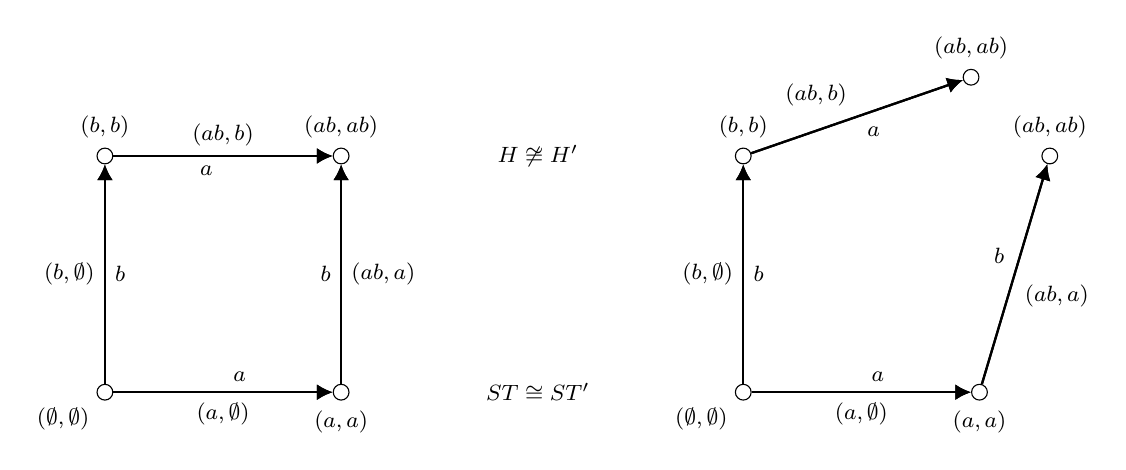
\begin{tikzpicture}[node distance=3cm, align=center]
  \tikzstyle{every node}=[font=\footnotesize]
    \tikzstyle{every state}=[fill=white,shape=circle,inner sep=.5mm,minimum size=3mm]
    \title{Strong asymmetric conflict a + b}
    
    \node[state](q1) [label=below left:{$(\emptyset, \emptyset)$}]      {};
    \node[state](q2) [right of=q1, label=below:{$(a,a)$}]               {};
    \node[state](q3) [above of=q1, label={$(b,b)$}]                     {};
    \node[state](q4) [above of=q2, label=above:{$(ab,ab)$}]             {};
    
    \node[state](q11) [right=8cm, label=below left:{$(\emptyset, \emptyset)$}]      {};
    \node[state](q22) [right of=q11, label=below:{$(a,a)$}]                         {};
    \node[state](q33) [above of=q11, label={$(b,b)$}]                               {};
    \node[state](q44) at (11, 4) [label=above:{$(ab,ab)$}]                          {};
    \node[state](q55) at (12, 3) [label=above:{$(ab,ab)$}]                          {};
    
    
    %%%% HDA isomorphism
    \node(HDA) at (5.5, 3)  {$H \not\cong H'$};
    
    %%%% ST-structure isomorphism
    \node(ST) at (5.5, 0)  {$ST \cong ST'$};
    
    %%%% Left figure
    \draw [->][draw=black, thick] (q1) to node [right] {$b$} (q3);
    \draw [->][draw=black, thick] (q1) to node [left] {$(b,\emptyset)$} (q3);
    \draw [->][draw=black, thick] (q1) to node [below] {$(a,\emptyset)$} (q2);
    \draw [->][draw=black, thick] (q1) to node [above right] {$a$} (q2);
    \draw [->][draw=black, thick] (q3) to node [above] {$(ab,b)$} (q4);
    \draw [->][draw=black, thick] (q3) to node [below left] {$a$} (q4);
    \draw [->][draw=black, thick] (q2) to node [left] {$b$} (q4);
    \draw [->][draw=black, thick] (q2) to node [right] {$(ab,a)$} (q4);
    
    
    %%%% Right figure
    \draw [->][draw=black, thick] (q11) to node [right] {$b$} (q33);
    \draw [->][draw=black, thick] (q11) to node [left] {$(b,\emptyset)$} (q33);
    \draw [->][draw=black, thick] (q11) to node [below] {$(a,\emptyset)$} (q22);
    \draw [->][draw=black, thick] (q11) to node [above right] {$a$} (q22);
    \draw [->][draw=black, thick] (q33) to node [above left] {$(ab,b)$} (q44);
    \draw [->][draw=black, thick] (q33) to node [below right] {$a$} (q44);
    \draw [->][draw=black, thick] (q22) to node [above left] {$b$} (q55);
    \draw [->][draw=black, thick] (q22) to node [below right] {$(ab,a)$} (q55);
    

  \end{tikzpicture}
\end{document}